\renewcommand{\thesection}{\Roman{section}}
\titleformat{\section}
{\normalfont\bfseries}{PHẦN~\thesection.}{0.4em}{}
\newcolumntype{C}[1]{>{\centering\arraybackslash}p{#1}}
\newcolumntype{L}[1]{>{\raggedright\arraybackslash}p{#1}}
\begin{tabular}{C{5cm}C{11cm}}
	\textbf{TRUNG TÂM MANABIE}& \textbf{ĐỀ ÔN TẬP KIỂM TRA GIỮA HỌC KÌ 2} \\
	\textbf{ĐỀ 02}& \textbf{Môn: VẬT LÝ}\\
	\textit{(Đề có 05 trang)}& \textit{Thời gian làm bài: 50 phút, không kể thời gian phát đề}
	
	\noindent\rule{4cm}{0.8pt} \\
\end{tabular}
\hdc{
	\section{}
	Mỗi câu trả lời đúng thí sinh được \textbf{0,25 điểm}.
	\begin{center}
		\begin{tabular}{|C{2.5cm}|C{4.0cm}|C{2.5cm}|C{4.0cm}|}
			\hline
			\thead{Câu} & \thead{Đáp án} & \thead{Câu} & \thead{Đáp án}\\
			\hline
			1 & C &  10 & B \\ 
			\hline
			2 & A &  11 & D \\ 
			\hline
			3 & B &  12 & C \\ 
			\hline
			4 & D &  13 & B \\ 
			\hline
			5 & B &  14 & B \\ 
			\hline
			6 & D &  15 & B \\ 
			\hline
			7 & A &  16 & C \\ 
			\hline
			8 & B &  17 & A \\ 
			\hline
			9 & A &  18 & A \\ 
			\hline
		\end{tabular}
	\end{center}
	\section{}
	Điểm tối đa của 01 câu hỏi là \textbf{1 điểm}.
	\begin{itemize}
		\item Thí sinh lựa chọn chính xác 01 ý trong 1 câu hỏi được \textbf{0,1} điểm.
		\item Thí sinh lựa chọn chính xác 02 ý trong 1 câu hỏi được \textbf{0,25} điểm.
		\item Thí sinh lựa chọn chính xác 03 ý trong 1 câu hỏi được \textbf{0,50} điểm.
		\item Thí sinh lựa chọn chính xác cả 04 ý trong 1 câu hỏi được \textbf{1} điểm.
	\end{itemize}
	\begin{center}
		\begin{tabular}{|C{1.0cm}|C{2.0cm}|C{3.0cm}|C{1.0cm}|C{2.0cm}|C{3.0cm}|}
			\hline
			\thead{Câu} & \thead{Lệnh hỏi} &\thead{Đáp án\\ (Đ/S)} &\thead{Câu} & \thead{Lệnh hỏi} &\thead{Đáp án\\ (Đ/S)}\\
			\hline
			\multirow{4}{*}{\textbf{1}}& a) & S & \multirow{4}{*}{\textbf{3}} & a) & S \\
			\cline{2-3}\cline{5-6}
			& b) & S &                             & b) & Đ \\
			\cline{2-3}\cline{5-6}
			& c) & Đ &                             & c) & S \\
			\cline{2-3}\cline{5-6}
			& d) & S &                             & d) & Đ \\
			\hline
			\multirow{4}{*}{\textbf{2}}& a) & Đ & \multirow{4}{*}{\textbf{4}} & a) & Đ \\
			\cline{2-3}\cline{5-6}
			& b) & S &                             & b) & S \\
			\cline{2-3}\cline{5-6}
			& c) & Đ &                             & c) & Đ \\
			\cline{2-3}\cline{5-6}
			& d) & Đ &                             & d) & Đ \\
			\hline		                           		                       
		\end{tabular}
	\end{center}
	\section{}
	Mỗi câu trả lời đúng thí sinh được \textbf{0,25 điểm}.
	\begin{center}
		\begin{tabular}{|C{2.5cm}|C{4.0cm}|C{2.5cm}|C{4.0cm}|}
			\hline
			\thead{Câu} & \thead{Đáp án} & \thead{Câu} & \thead{Đáp án}\\
			\hline
			1 & $1/3$ &  4 & 13,26 \\ 
			\hline
			2 & 377,69 &  5 & 1,2 \\ 
			\hline
			3 & 1000 &  6 & 160 \\ 
			\hline
		\end{tabular}
	\end{center}
	\newpage
}
\setcounter{section}{0}
\section{Câu trắc nghiệm nhiều phương án lựa chọn.}
\textit{Thí sinh trả lời từ câu 1 đến câu 18. Mỗi câu hỏi thí sinh chọn một phương án.}
\begin{enumerate}[label=\bfseries Câu \arabic*:]
	\item Câu phát biểu nào sau đây đúng?
	\begin{mcq}
		\item Electron là hạt sơ cấp mang điện tích nguyên tố $\SI{1.6E-19}{\coulomb}$.
		\item Độ lớn của điện tích nguyên tố là $\SI{1.6E19}{\coulomb}$.
		\item Điện tích hạt nhân bằng bằng một số nguyên lần điện tích nguyên tố.
		\item Tất cả các hạt sơ cấp đều mang điện tích.
	\end{mcq}
\hideall{
\textbf{Đáp án C.}
}

\item Cho một điện tích di chuyển trong điện trường dọc theo một đường cong kín, xuất phát từ điểm M qua điểm N rồi trở lại điểm M. Chọn phát biểu đúng.
\begin{mcq}
	\item Công của lực điện trong cả quá trình bằng 0.
	\item Công của lực điện trong quá trình M đến N là dương.
	\item Công của lực điện trong quá trình N đến M là dương.	
	\item Công của lực điện trong cả quá trình là dương.
\end{mcq}
\hideall{
\textbf{Đáp án A.}\\
Điểm đầu và điểm cuối cùng trùng nhau nên $A = 0$.
}

\item Công của lực điện tác dụng lên một điện tích điểm q khi di chuyển từ điểm M đến điểm N trong điện trường?
\begin{mcq}
	\item Tỉ lệ thuận với chiều dài đường đi MN.
	\item Tỉ lệ thuận với độ lớn của điện tích $q$.
	\item Tỉ lệ thuận với thời gian di chuyển.
	\item Tỉ lệ thuận với tốc độ dịch chuyển.
\end{mcq}
\hideall{
\textbf{Đáp án B.}\\
$$A_\text{MN}=q\left(V_\text{M}-V_\text{N}\right).$$
}
	
	\item Hai điện $q_1<0$ và $q_2>0$ với $\left|q_2\right|>\left|q_1\right|$ lần lượt đặt tại hai điểm A và B như hình vẽ (I là trung điểm của AB). Điểm M có cường độ điện trường tổng hợp do hai điện tích này gây ra bằng 0 nằm trên
	\begin{center}
		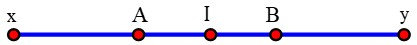
\includegraphics[width=0.4\linewidth]{../figs/PH11-MidSem2-02-1}
	\end{center}
\begin{mcq}(4)
	\item AI.
	\item IB.
	\item Bv.
	\item Ax.
\end{mcq}
\hideall{
\textbf{Đáp án D.}\\
Các điện trường thành phần phải cùng phương ngược nhiều và cùng độ lớn, điều này chỉ có thể xảy ra khi M nằm ngoài AB.\\
Mà $\left|q_2\right|>\left|q_1\right|$ nên $\text{MB}>\text{MA}$.
}

\item Vào mùa hanh khô, nhiều khi kéo áo len qua đầu, ta nghe thấy có tiếng nổ lách tách. Đó là do
\begin{mcq}(2)
	\item Hiện tượng nhiễm điện do tiếp xúc.
	\item Hiện tượng nhiễm điện do cọ xát.
	\item Hiện tượng nhiễm điện do hưởng ứng.
	\item Cả ba hiện tượng nhiễm điện trên.
\end{mcq}
\hideall{
\textbf{Đáp án B.}\\
Hiện tượng trên là hiện tượng nhiễm điện do sự cọ xát của tóc và áo len.
}

\item Đưa một thanh kim loại trung hoà về điện đặt trên một giá cách điện lại gần một quả cầu tích điện dương. Sau khi đưa thanh kim loại ra thật xa quả cầu thì thanh kim loại
\begin{mcq}(2)
	\item có hai nửa tích điện trái dấu.
	\item tích điện dương.
	\item tích điện âm.
	\item trung hoà về điện.
\end{mcq}
\hideall{
\textbf{Đáp án D.}
}

\item Hai quả cầu kim loại nhỏ A và B giống hệt nhau, được treo vào một điểm O bằng hai sợi chi dài bằng nhau. Khi cân bằng, ta thấy hai sợi chỉ làm với đường thẳng đững những góc $\alpha$ bằng nhau (xem hình vẽ). Trạng thái nhiễm điện của hai quả cầu sẽ là trạng thái nào đây? 
\begin{center}
	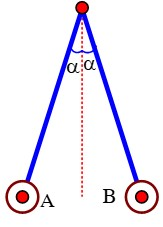
\includegraphics[width=0.2\linewidth]{../figs/PH11-MidSem2-02-2}
\end{center}
\begin{mcq}
	\item Hai quả cầu nhiễm điện cùng dấu.
	\item Hai quả cầu nhiễm điện trái dấu. 
	\item Hai quả cầu không nhiễm điện.
	\item Một quả cầu nhiễm điện, một quả cầu không nhiễm điện.
\end{mcq}
\hideall{
\textbf{Đáp án A.}
}

\item Nhiễm điện cho một thanh nhựa rồi đưa nó lại gần hai vật M và N. Ta thấy thanh nhựa hút cả hai vật M và N. Tình huống nào dưới đây chắc chắn không thể xảy ra?
\begin{mcq}(2)
	\item M và N nhiễm điện cùng dấu.	
	\item M và N nhiễm điện trái dấu.
	\item M nhiễm điện, còn N không nhiễm điện.
	\item Cả M và N đều không nhiễm điện.
\end{mcq}
\hideall{
\textbf{Đáp án B.}\\
Nếu hai vật nhiễm điện trái dấu thì sẽ có một vật bị hút và một vật bị đẩy.
}

\item Treo một sợi tóc trước màn hình của một máy thu hình (ti vi) chưa hoạt động. Khi bật tivi thì thành thủy tinh ở màn hình
\begin{mcq}
	\item nhiễm điện nên nó hút sợi dây tóc.
	\item nhiễm điện cùng  dấu với sợi dây tóc nên nó đẩy sơi tóc.
	\item không nhiễm điện nhưng sợi dây tóc nhiễm điện âm nên sợi dây tóc duỗi thẳng.
	\item không nhiễm điện nhưng sợi dây tóc nhiễm điện dương nên sợi tóc duỗi thẳng.
\end{mcq}
\hideall{
\textbf{Đáp án A.}\\
Thành thủy tinh ở màn hình nhiễm điện nên nó hút sợi tóc.
}

\item Đại lượng nào dưới đây không liên quan đến cường độ điện trường của một điện tích điểm $Q$ gây ra tại một điểm?
\begin{mcq}(2)
	\item Điện tích $Q$.
	\item Điện tích thử $q$.
	\item Khoảng cách từ $Q$ đến điểm đang xét.
	\item Hằng số điện môi của môi trường.
\end{mcq}
\hideall{
\textbf{Đáp án B.}
}

\item Ba điện tích điểm $q_1=\SI{3E-8}{\coulomb}$ nằm tại điểm A; $q_2=\SI{4E-8}{\coulomb}$ nằm tại điểm B và $q_3=\SI{-0.684E-8}{\coulomb}$ nằm tại điểm C. Hệ thống nằm cân bằng trên mặt phẳng nhẵn nằm ngang. Độ lớn cường độ điện trường tại các điểm A, B và C lần lượt là $E_\text{A}$, $E_\text{B}$ và $E_\text{C}$. Chọn phương án \textbf{đúng}?
\begin{mcq}(2)
	\item $E_\text{A}>E_\text{B}=E_\text{C}$.
	\item $E_\text{A}>E_\text{B}>E_\text{C}$.
	\item $E_\text{A}<E_\text{B}=E_\text{C}$.
	\item $E_\text{A}=E_\text{B}=E_\text{C}.$
\end{mcq}
\hideall{
\textbf{Đáp án D.}\\
Vì hệ cân bằng nên điện trường tổng hợp tại A, B và C đều bằng 0.
}

\item Trên hình bên có vẽ một số đường sức của hệ thống hai điện tích điểm. Các điện tích đó là
\begin{center}
	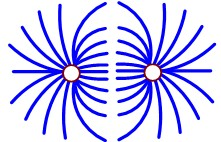
\includegraphics[width=0.3\linewidth]{../figs/PH11-MidSem2-02-3}
\end{center}
\begin{mcq}
	\item hai điện tích dương.
	\item hai điện tích âm.
	\item một điện tích dương, một điên tích âm.
	\item không thể có các đường sức có dạng như thế.
\end{mcq}
\hideall{
\textbf{Đáp án C.}\\
 Đường sức của điện tích điểm âm hướng về điện tích đó còn điện tích dương hướng ra khỏi điện tích đó.
}

\item Một điện tích điểm $Q=\SI{-2E-7}{\coulomb}$ đặt tại điểm A trong môi trường có hằng số điện môi $\varepsilon=2$. Vector cường độ điện trường do điện tích $Q$ gây ra tại điểm B với $\text{AB}=\SI{7.5}{\centi\meter}$ có
\begin{mcq}
	\item phương AB, chiều từ A đến B, độ lớn $\SI{2.5E5}{\volt/\meter}$.
	\item phương AB, chiều từ B đến A, độ lớn $\SI{1.6E5}{\volt/\meter}$.
	\item phương AB, chiều từ B đến A, độ lớn $\SI{2.5E5}{\volt/\meter}$.
	\item phương AB, chiều từ A đến B, độ lớn $\SI{1.6E5}{\volt/\meter}$.
\end{mcq}
\hideall{
\textbf{Đáp án B.}\\
Điện tích âm nên chiều của điện trường có phương AB, chiều từ B đến A, độ lớn:
$$E=\dfrac{k\left|Q\right|}{\varepsilon r^2}=\SI{1.6E5}{\volt/\meter}.$$
}



\item Tính cường độ điện trường do một điện tích điểm $\SI{4E-9}{\coulomb}$ gây ra tại một điểm cách nó $\SI{5}{\centi\meter}$ trong chân không
\begin{mcq}(4)
	\item $\SI{144}{\kilo\volt/\meter}$.
	\item $\SI{14.4}{\kilo\volt/\meter}$.
	\item $\SI{288}{\kilo\volt/\meter}$.
	\item $\SI{28.8}{\kilo\volt/\meter}$.
\end{mcq}
\hideall{
\textbf{Đáp án B.}\\
Độ lớn cường độ điện trường do điện tích $Q$ gây ra:
$$E=\dfrac{k\left|Q\right|}{r^2}=\SI{14.4}{\kilo\volt/\meter}.$$
}

\item Lực hút tĩnh điện giữa hai điện tích là $\SI{2E-6}{\newton}$. Khi đưa chúng xa nhau thêm $\SI{2}{\centi\meter}$ thì lực hút là $\SI{5E-7}{\newton}$. Khoảng cách ban đầu giữa chúng là
\begin{mcq}(4)
	\item $\SI{1}{\centi\meter}$.
	\item $\SI{2}{\centi\meter}$.
	\item $\SI{3}{\centi\meter}$.
	\item $\SI{4}{\centi\meter}$.
\end{mcq}
\hideall{
\textbf{Đáp án B.}\\
$$\begin{cases}
	F=\dfrac{k\left|q_1q_2\right|}{r^2}\\
	F'=\dfrac{k\left|q_1q_2\right|}{\left(r+0,02\right)^2}
\end{cases}
\Rightarrow \dfrac{F'}{F}=\dfrac{\left(r+0,02\right)^2}{r^2}\Rightarrow r=\SI{0.02}{\meter}.$$
}

\item Một quả cầu nhỏ có khối lượng $m=\SI{0.1}{\kilogram}$ được treo ở đầu một sợi chỉ mảnh, trong một điện trường đều, có phương nằm ngang và có cường độ điện trường $E=\SI{E3}{\volt/\meter}$. Dây chỉ hợp với phương thẳng đứng một góc $\SI{14}{\degree}$. Tính độ lớn điện tích của quả cầu. Lấy $g=\SI{10}{\meter/\second^2}$.
\begin{mcq}(4)
	\item $\SI{0.176}{\micro\coulomb}$.
	\item $\SI{0.276}{\micro\coulomb}$.
	\item $\SI{0.249}{\micro\coulomb}$.
	\item $\SI{0.272}{\micro\coulomb}$.
\end{mcq}
\hideall{
	\textbf{Đáp án C.}\\
	\begin{center}
		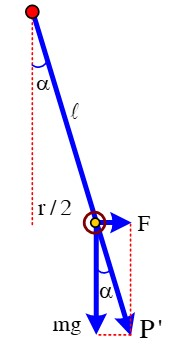
\includegraphics[width=0.2\linewidth]{../figs/PH11-MidSem2-02-4}
	\end{center}
	Khi hệ cân bằng thì $\vec{F}+\vec{P}+\vec{T}=\vec{0}$.
	Ta có:
	$$\tan\alpha=\dfrac{F}{mg}=\dfrac{\left|q\right|E}{mg}$$
	$$\Rightarrow \left|q\right|=\dfrac{mg\tan\alpha}{E}=\SI{0.249}{\micro\coulomb}.$$
}

\item Một electron chuyển động với vận tốc ban đầu $\SI{2E6}{\meter/\second}$ dọc theo một đường sức điện của một điện trường đều được một quãng đường $\SI{1}{\centi\meter}$ thì dừng lại. Điện tích của electron là $\SI{-1.6E-19}{\coulomb}$, khối lượng của electron là $\SI{9.1E-31}{\kilogram}$. Độ lớn cường độ điện trường trên là
\begin{mcq}(4)
	\item $\SI{1137.5}{\volt/\meter}$.
	\item $\SI{144}{\volt/\meter}$.
	\item $\SI{284}{\volt/\meter}$.
	\item $\SI{1175.5}{\volt/\meter}$.
\end{mcq}
\hideall{
\textbf{Đáp án A.}\\
Electron chuyển động chậm dần nên lực tĩnh điện tác dụng lên electron ngược chiều vector vận tốc đầu.\\
Áp dụng định lý động năng cho quá trình chuyển động của electron
$$0-\dfrac{1}{2}mv^2_0=\left|e\right|Es\cos\SI{180}{\degree}$$
$$\Rightarrow E=\dfrac{mv^2}{2\left|e\right|s}=\SI{1137.5}{\volt/\meter}.$$
}

\item Tại điểm O đặt điện tích $Q$. Trên tia $Ox$ có ba điểm theo đúng thứ tự A, M, B. Độ lớn cường độ điện trường tại điểm A, M, B lần lượt là $E_\text{A}$, $E_\text{M}$ và $E_\text{B}$. Nếu $E_\text{A}=\SI{96100}{\volt/\meter}$, $E_\text{B}=\SI{5625}{\volt/\meter}$ và $\text{MA}=2\text{MB}$ thì $E_\text{M}$ \textbf{gần nhất với giá trị nào} sau đây?
\begin{mcq}(4)
	\item $\SI{10072}{\volt/\meter}$.
	\item $\SI{22000}{\volt/\meter}$.
	\item $\SI{11200}{\volt/\meter}$.
	\item $\SI{10500}{\volt/\meter}$.
\end{mcq}
\hideall{
\textbf{Đáp án A.}\\
Từ $\text{MA}=2\text{MB}\Rightarrow r_\text{M}-r_\text{A}=2\left(r_\text{B}-r_\text{M}\right)\Rightarrow 3r_\text{M}=r_\text{A}+2r_\text{B}$
Vì $E=\dfrac{k\left|Q\right|}{\varepsilon r^2}\Rightarrow r\sim\dfrac{1}{\sqrt{E}}$.\\
$$\dfrac{3}{\sqrt{E_\text{M}}}=\dfrac{1}{\sqrt{E_\text{A}}}+\dfrac{2}{\sqrt{E_\text{B}}}\Rightarrow E_\text{M}=\SI{10072}{\volt/\meter}.$$
}
\end{enumerate}
\section{Câu trắc nghiệm đúng sai.} 
\textit{Thí sinh trả lời từ câu 1 đến câu 4. Trong mỗi ý \textbf{a)}, \textbf{b)}, \textbf{c)}, \textbf{d)} ở mỗi câu, thí sinh chọn đúng hoặc sai.}
\begin{enumerate}[label=\bfseries Câu \arabic*:]
	\item Nhận định về các phát biểu sau:
	\begin{enumerate}[label=\bfseries \alph*)]
		\item Điện thế tại một điểm trong điện trường được xác định bằng công lực điện dịch chuyển một đơn vị điện tích dương từ vô cùng về điểm đó.
		\item Vector cường độ điện trường hướng từ nơi điện thế thấp về nơi điện thế cao.
		\item Hiệu điện thế giữa hai điểm bất kì trong điện trường không phụ thuộc gốc điện thế.
		\item Đơn vị điện thế là joule $\left(\si{\joule}\right)$.
	\end{enumerate}
\hideall{
\begin{enumerate}[label=\bfseries \alph*)]
	\item Sai. Điện thế tại một điểm trong điện trường được xác định bằng công lực điện dịch chuyển một đơn vị điện tích dương điểm đó ra xa vô cùng.
	\item Sai. Vector cường độ điện trường hướng từ nơi điện thế cao sang nơi điện thế thấp.
	\item Đúng.
	\item Sai. Đơn vị điện thế là volt $\left(\si{\joule}\right)$.
\end{enumerate}
}
 
 \item Tụ điện phẳng có điện dung $\SI{2}{\micro\farad}$ và được tích điện dưới hiệu điện thế $\SI{120}{\volt}$. Sau khi nạp điện, tụ được ngắt khỏi nguồn và người ta tăng khoảng cách giữa hai bản của tụ lên gấp đôi.
 \begin{enumerate}[label=\bfseries \alph*)]
 	\item Điện tích của tụ sau khi nạp điện là $\SI{240}{\micro\coulomb}$.
 	\item Sau khi tăng khoảng cách giữa hai bản thì điện tích của tụ là $\SI{120}{\micro\coulomb}$.
 	\item Điện dung của tụ sau khi tăng khoảng cách sẽ giảm đi 2 lần.
 	\item Công cần thực hiện để thay đổi khoảng cách giữa hai bản tụ là $\SI{0.0144}{\joule}$.
 \end{enumerate}
\hideall{
\begin{enumerate}[label=\bfseries \alph*)]
	\item Đúng.
	\item Sai. Điện tích của tụ không đổi.
	\item Đúng. Điện dung tụ điện phẳng $C\sim \dfrac{1}{d}$.
	\item Đúng. Công cần thực hiện để tăng khoảng cách giữa hai bản lên gấp đôi:
	$$A=\dfrac{1}{2}\dfrac{q^2}{C'}-\dfrac{1}{2}\dfrac{q^2}{C}=\dfrac{1}{2}\dfrac{q^2}{C}=\SI{0.0144}{\joule}.$$
\end{enumerate}
}

	\item Thí nghiệm giọt dầu của Millikan là thí nghiệm đầu tiên xác định được điện tích nguyên tố. Trong đó, giọt dầu lơ lửng ở giữa không gian 2 bản phẳng tích điện trái dấu (như hình vẽ) nhờ lực tĩnh điện cân bằng với trọng lực của giọt dầu. Giọt dầu hình cầu có bán kính $\SI{1}{\micro\meter}$ và có khối lượng riêng $\SI{920}{\kilogram/\meter^3}$. Gia tốc trọng trường tại nơi làm thí nghiệm $g=\SI{9.8}{\meter/\second^2}$.
	\begin{center}
		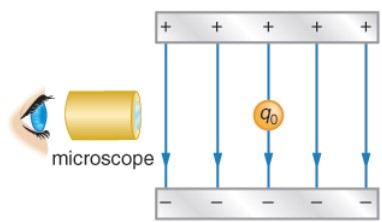
\includegraphics[width=0.4\linewidth]{../figs/PH11-MidSem2-02-6}
	\end{center}
	\begin{enumerate}[label=\bfseries \alph*)]
		\item Giọt dầu tích điện dương.
		\item Trọng lượng giọt dầu là $\SI{3.78E-14}{\newton}$.
		\item Nếu giọt dầu có thừa 1 electron thì cường độ điện trường để giữ giọt dầu cân bằng là $\SI{236}{\volt}$.
		\item Nếu đảo chiều điện trường thì giọt dầu rơi nhanh dần đều.
	\end{enumerate}
\hideall{
\begin{enumerate}[label=\bfseries \alph*)]
	\item Sai. Lực điện ngược chiều điện trường nên giọt dầu phải tích điện âm.
	\item Đúng. Trọng lượng giọt dầu:
	$$P=\rho gV=\dfrac{4}{3}\pi r^3\rho g=\SI{3.78E-14}{\newton}.$$
	\item Sai. Để giọt dầu cân bằng thì:
	$$F_\text{đ}=P\Leftrightarrow \left|e\right|E=P\Rightarrow E=\dfrac{P}{\left|E\right|}\approx\SI{236}{\kilo\volt}.$$
	\item Đúng. $\vec{F}_\text{đ}\uparrow\uparrow\vec P$.
\end{enumerate}
}
	\item Hình bên mô tả chuyển động của một electron khi đi qua vùng không gian giữa hai bản kim loại phẳng, tích điện trái dâu với cường độ điện trường giữa hai bản là $\SI{100}{\newton/\coulomb}$. Ban đầu, electron bay theo phương song song hai bản với tốc độ $\SI{3.00E6}{\meter/\second}$. Electron di chuyển đươc quãng đường $\SI{4.00}{\centi\meter}$ theo phương ngang trước khi rời khỏi hai bản. Khối lượng và điện tích của electron lần lượt là $\SI{9.11E-31}{\kilogram}$ và $\SI{-1.60E-19}{\coulomb}$.
	\begin{center}
		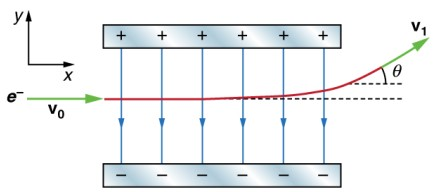
\includegraphics[width=0.5\linewidth]{../figs/PH11-MidSem2-02-5}
	\end{center}
	\begin{enumerate}[label=\bfseries \alph*)]
		\item Khi rời khỏi hai vùng không gian giữa hai bản, tốc độ của electron trên phương ngang là $\SI{3E6}{\meter/\second}$.
		\item Thời gian electron chuyển động trong vùng không gian giữa hai bản là $\SI{1.33}{\micro\second}$.
		\item Độ lệch của electron theo phương thẳng đứng là $\SI{1.56}{\milli\meter}$.
		\item Góc lệch $\theta\approx\SI{4.5}{\degree}$.
	\end{enumerate}
\hideall{
\begin{enumerate}[label=\bfseries \alph*)]
	\item Đúng.
	\item Sai. Thời gian chuyển động trong vùng điện trường:
	$$t=\dfrac{s}{v_0}=\SI{1.33E-8}{\second}.$$
	\item Đúng. Độ lệch của electron theo phương thẳng đứng:
	$$h=\dfrac{1}{2}a_yt^2=\dfrac{1}{2}\left(\dfrac{\left|e\right|E}{m_e}\right)\cdot\left(\dfrac{s}{v_0}\right)^2=\SI{1.56E-3}{\meter}.$$
	\item Đúng. Góc lệch $\theta$:
	$$\tan\theta=\dfrac{v_y}{v_x}=\dfrac{\dfrac{\left|e\right|Et}{m_e}}{v_0}\approx0,078\Rightarrow\theta=\SI{4.5}{\degree}.$$
\end{enumerate}
}
\end{enumerate}
\section{Câu trắc nghiệm trả lời ngắn.} \textit{Thí sinh trả lời từ câu 1 đến câu 6.}
\begin{enumerate}[label=\bfseries Câu \arabic*:]
	\item Một quả cầu kim loại A mang điện dương $q$ được đặt tại nơi có cường độ điện trườn $E$ thì chịu tác dụng của lực điện có độ lớn $F$. Cho quả cầu kim loại B mang điện dương $Q$ tiếp xúc quả cầu A, sau đó đưa quả cầu B ra xa. Lúc này lực điện tác dụng lên quả cầu A là $2F$. Biết rằng hai quả cầu hoàn toàn giống nhau. Tỉ số độ lớn giữa $q$ và $Q$ là bao nhiêu?
	\hideall{
	Sau khi tiếp xúc, lực điện tác dụng lên quả cầu A tăng gấp đôi $\Rightarrow q'=2q$.\\
	Điện tích của quả cầu A sau khi tiếp xúc quả cầu B:
	$$q'=\dfrac{q+Q}{2}=2q$$
	$$\Rightarrow \dfrac{q}{Q}=\dfrac{1}{3}.$$
}
	\item Trong chân không có ba điểm A, B, C tạo thành một tam giác vuông tại A có $\text{AB}=\SI{12}{\centi\meter}$, $\text{AC}=\SI{20}{\centi\meter}$. Tại B đặt điện tích $q_1=\SI{6E-7}{\coulomb}$, tại C đặt điện tích $q_2=\SI{2E-7}{\coulomb}$. Cường độ điện trường tổng hợp do hai điện tích gây ra tại A là bao nhiêu $\si{\kilo\volt/\meter}$ \textit{(kết quả tính đến 2 chữ số thập phân)}?
\hideall{
	Cường độ điện trường do điện tích tại B gây ra tại A:
	$$E_1=\dfrac{k\left|q_1\right|}{AB^2}=\SI{3.75E5}{\volt/\meter}.$$
	Cường độ điện trường do điện tích tại C, gây ra tại A:
	$$E_2=\dfrac{k\left|q_2\right|}{AC^2}=\SI{0.45E5}{\volt/\meter}.$$
	Cường độ điện trường tổng hợp do hai điện tích gây ra tại A:
	$$E=\sqrt{E^2_1+E^2_2}\approx\SI{377.69}{\kilo\volt/\meter}.$$
}

\item Một điện tích $q=\SI{2E-8}{\coulomb}$ khi dịch chuyển từ M đến N thì lực điện trường thực hiện công $A_\text{MN}=\SI{2E-5}{\joule}$. Hiệu điện thế giữa hai điểm MN là bao nhiêu volt?
\hideall{
Hiệu điện thế giữa hai điểm MN:
$$U_\text{MN}=\dfrac{A_\text{MN}}{q}=\SI{1000}{\volt}.$$
}

\item Một proton bắt đầu chuyển động không vận tốc đầu trong một điện trường đều có cường độ $E=\SI{2500}{\volt/\meter}$ dọc theo đường sức điện và cùng chiều đường sức. Tốc độ của proton khi nó đi được quãng đường $\SI{20}{\centi\meter}$ là $\xsi{x\cdot 10^6}{\meter/\second}$. Biết khối lượng proton là $m_p=\SI{1.67E-27}{\kilogram}$. Xác định giá trị của $x$ \textit{(làm tròn đến 2 chữ số thập phân)}.
\hideall{
Áp dụng định lý động năng cho quá trình chuyển động của proton trong điện trường:
$$\dfrac{1}{2}m_pv^2-0=qEs$$
$$\Rightarrow v=\sqrt{\dfrac{2qEs}{m_p}}=\SI{13.26E6}{\meter/\second}.$$
}

\item Một quả cầu kim loại tich điện $q=\SI{5}{\micro\coulomb}$ được đặt cách mặt đất $\SI{2}{\meter}$. Biết điện trường ở gần mặt đất xem như điện trường đều hướng xuống có độ lớn $E=\SI{120}{\volt/\meter}$. Lấy gốc thế năng tại mặt đất, tính thế năng của điện tích trên \textit{(tính theo đơn vị $\si{\milli\joule}$)}.
\hideall{
Lấy gốc thế năng ở mặt đất.\\
Thế năng của điện tích trong điện trường:
$$W=qEd=\SI{1.2}{\milli\joule}.$$
}

\item Có 3 tụ điện $C_1=\SI{2}{\micro\farad}$, $C_2=\SI{4}{\micro\farad}$ và $C_3=\SI{8}{\micro\farad}$ được ghép nối tiếp với nhau. Khi đặt bộ tụ vào hiệu điện thế $U=\SI{140}{\volt}$. Tính điện tích trên các tụ điện \textit{(theo đơn vị $\si{\micro\coulomb}$)}.
\hideall{
	Điện dung của bộ tụ điện:
	$$\dfrac{1}{C}=\dfrac{1}{C_1}+\dfrac{1}{C_2}+\dfrac{1}{C_3}\Rightarrow  C=\xsi{\dfrac{8}{7}}{\micro\farad}.$$
	Điện tích của bộ tụ điện:
	$$Q=CU=\SI{160}{\micro\coulomb}.$$
}
\begin{center}
	\textbf{--- HẾT ---}
\end{center}
\end{enumerate}